\begin{exercise}
      {ID-b75ee6a9f0c1b08630cdb754aa7c8602714f4880}
      {Klebeband}
  \ifproblem\problem
    \begin{minipage}{0.33\linewidth}
      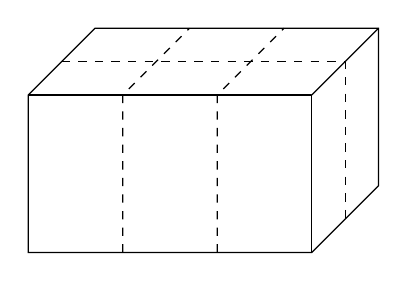
\begin{tikzpicture}[scale=0.8]
        \draw (0, 0)
              -- ++(0:45mm)
              -- ++(45:15mm)
              -- ++(90:25mm) coordinate (A)
              -- ++(180:45mm)
              -- ++(225:15mm)
              -- cycle;
        \begin{scope}[line join=bevel]
          \draw (0, 25mm) -- (45mm, 25mm) -- (45mm, 0);
          \draw (45mm, 25mm) -- (A);
        \end{scope}
        \begin{scope}[line join=bevel, style=dashed]
          \draw[shift={(45:7.5mm)}] (0, 25mm) -- (45mm, 25mm) -- (45mm, 0);
          \draw[xshift=15mm] (0, 0)  -- (0, 25mm) -- ++(45:15mm);
          \draw[xshift=30mm] (0, 0)  -- (0, 25mm) -- ++(45:15mm);
        \end{scope}
      \end{tikzpicture}%
    \end{minipage}\hfill
    \begin{minipage}{0.65\linewidth}
      Das in der Abbildung abgebildete Paket ist von links nach rechts \sicm{45}
      lang, von vorn nach hinten \sicm{30} breit, und es ist \sicm{25} hoch.
      Es soll in der dargestellten Weise (gestrichelte Linie) mit Klebeband
      verklebt werden. Für das Überlappen von End- und Anfangsstücken sind
      zusätzlich insgesamt \sicm{10} Klebeband vorgesehen.\par
      Wie viel Zentimeter Klebeband werden demnach insgesamt gebraucht?
      Wie viel Meter sind das?
    \end{minipage}
  \fi
  %\ifoutline\outline
  %\fi
  \ifoutcome\outcome
    Zum Verkleben des Paketes werden insgesamt \sicm{370} Klebeband benötigt.
    Das sind \simeter{3.70}.
  \fi
\end{exercise}
